% Generated by support/export-artifacts.py; do not edit.
% Slug: ch58-data
% Source: chapters/ch58.tex:114
% TikZ source: chapters/ch58.tex:116
% Original label: \label{fig:ch58-data}
% Original caption (LaTeX source):
%   The loader supplies the zero tail, including alignment before BSS, without reading forty additional payload bytes.
% Caption: The loader supplies the zero tail, including alignment before BSS, without reading forty additional payload bytes.
% Setup: support/compiler-pseudocode.sty (TikZ libraries and shared styles).
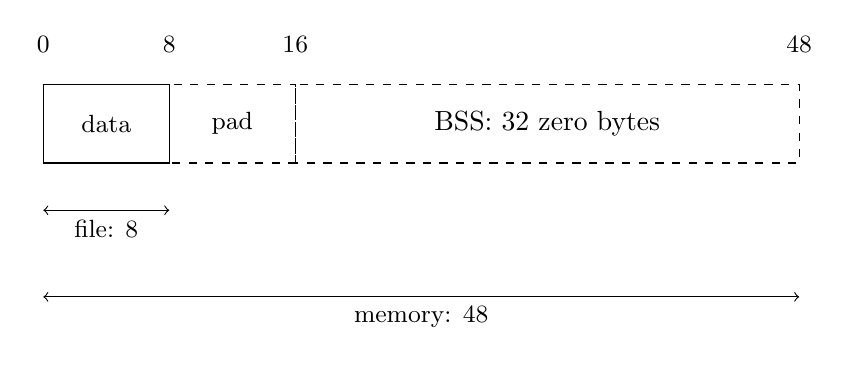
\begin{tikzpicture}[x=2mm,y=10mm]
\draw (0,0) rectangle (8,1); \node[font=\small] at (4,0.5) {data};
\draw[dashed] (8,0) rectangle (16,1); \node[font=\small] at (12,0.5) {pad};
\draw[dashed] (16,0) rectangle (48,1); \node at (32,0.5) {BSS: 32 zero bytes};
\draw[<->] (0,-0.6)--node[below,font=\small] {file: 8}(8,-0.6);
\draw[<->] (0,-1.7)--node[below,font=\small] {memory: 48}(48,-1.7);
\foreach \x in {0,8,16,48} \node[font=\small] at (\x,1.5) {\x};
\end{tikzpicture}

% Original figure LaTeX:
% \begin{figure}[htbp]
% \centering
% \begin{tikzpicture}[x=2mm,y=10mm]
% \draw (0,0) rectangle (8,1); \node[font=\small] at (4,0.5) {data};
% \draw[dashed] (8,0) rectangle (16,1); \node[font=\small] at (12,0.5) {pad};
% \draw[dashed] (16,0) rectangle (48,1); \node at (32,0.5) {BSS: 32 zero bytes};
% \draw[<->] (0,-0.6)--node[below,font=\small] {file: 8}(8,-0.6);
% \draw[<->] (0,-1.7)--node[below,font=\small] {memory: 48}(48,-1.7);
% \foreach \x in {0,8,16,48} \node[font=\small] at (\x,1.5) {\x};
% \end{tikzpicture}
% \caption{The loader supplies the zero tail, including alignment before BSS, without reading forty additional payload bytes.}
% \label{fig:ch58-data}
% \end{figure}
